\documentclass[sigconf]{acmart}
\usepackage{titlesec}
\setcopyright{none}
\acmConference[]{Deutschland, NRW, Düsseldorf}
\acmYear{}
\acmVolume{}
\acmNumber{}
\acmArticle{}
\copyrightyear{2020}
\acmISBN{}
\acmPrice{}
\acmSubmissionID{}
\acmDOI{}
\titlelabel{\upshape\thetitle\quad}
%%
%% \BibTeX command to typeset BibTeX logo in the docs
\AtBeginDocument{%
  \providecommand\BibTeX{{%
    \normalfont B\kern-0.5em{\scshape i\kern-0.25em b}\kern-0.8em\TeX}}}

\usepackage[ngerman]{babel}
\AfterEndEnvironment{equation}{\ignorespaces\newline}
\begin{document}
%%
%% The "title" command has an optional parameter,
%% allowing the author to define a "short title" to be used in page headers.
\title{Unicornn: Eine Unity Sprachsteuerung}

%%
%% The "author" command and its associated commands are used to define
%% the authors and their affiliations.
%% Of note is the shared affiliation of the first two authors, and the
%% "authornote" and "authornotemark" commands
%% used to denote shared contribution to the research.
\author{Alexander Pech (736825)}
\email{alexander.pech@study.hs-duesseldorf.de}
\affiliation{%
  \institution{Hochschule Düsseldorf}
}

\author{Lara Bertram (736057)}
\email{lara.bertram@study.hs-duesseldorf.de}
\affiliation{%
  \institution{Hochschule Düsseldorf}
}

\author{Alexander Mikulaschek (736306)}
\email{alexander.mikulaschek@study.hs-duesseldorf.de}
\affiliation{%
  \institution{Hochschule Düsseldorf}
}

\author{Philipp Jonas Knohl (710050)}
\email{philipp.jonas.knohl@study.hs-duesseldorf.de}
\affiliation{%
  \institution{Hochschule Düsseldorf}
}

%%
%% The abstract is a short summary of the work to be presented in the
%% article.
\begin{abstract}
Wir präsentieren eine einfache Sprachsteuerung für die Game Engine Unity 3D. Die Sprachsteuerung erkennt einzelne Wörter und klassifiziert diese mittels eines neuronalen Netzes. Bestimmte Kombinationen bei der Klassifizierung erlauben eine direkte Zuordnung zu Unity-Befehlen.  
Ein Beispiel wäre der Sprachbefehl ,,One“ + „Forward“, welcher in Unity „transform.position += Vector3.forward“ entspricht.
\newline
\newline
Bei dem neuronalen Netz handelt es sich um ein Convolutional Neural Network (kurz: CNN), da diese sich gut für Klassifizierungsaufgaben eignen. Teil dieser Arbeit ist dabei auch der Performanzvergleich zwischen VGG19 \cite{simonyan2014deep} und ResNet \cite{he2015deep} sowie die Verwendung des SGD- und Adam-Optimizers beim Trainingsprozess. 
Zur Demonstration des Projektes wurde eine Demoszene in Unity 3D erstellt, welche den Agenten enthält und es ermöglicht via Spracheingabe Objekt im Raum zu bewegen. 
\end{abstract}

%%
%% Keywords. The author(s) should pick words that accurately describe
%% the work being presented. Separate the keywords with commas.
\keywords{datasets, neural networks, speech recognition, Unity, Voice command}

%% A "teaser" image appears between the author and affiliation
%% information and the body of the document, and typically spans the
%% page.
\begin{teaserfigure}
  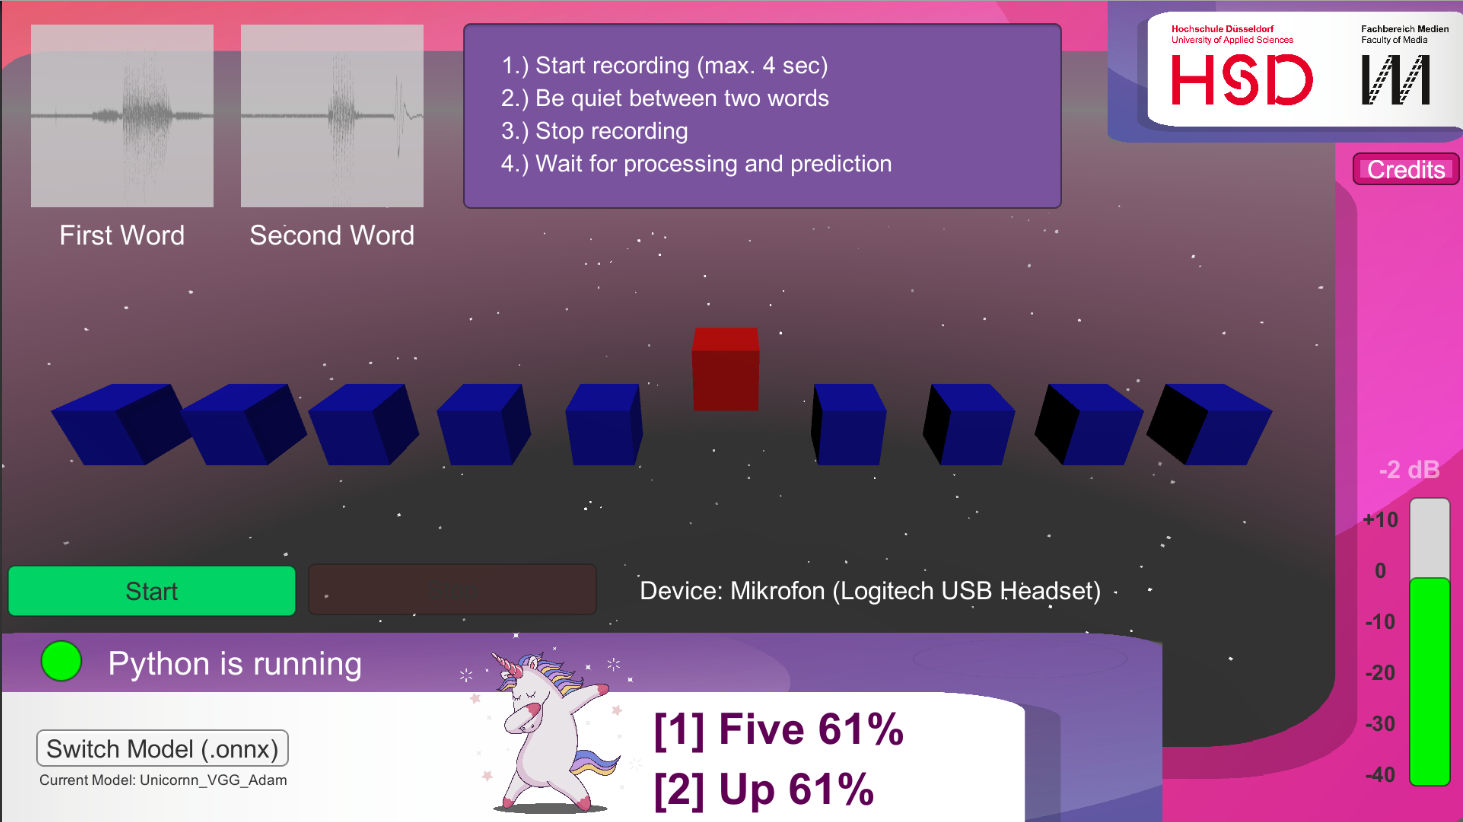
\includegraphics[width=\textwidth]{images/Demo}
  \caption{Screenshot des Interface der Unityanwendung.}
  \Description{Das Interface der Unity App.}
  \label{fig:UnityApp}
\end{teaserfigure}

%%
%% This command processes the author and affiliation and title
%% information and builds the first part of the formatted document.
\maketitle
\newpage
\section{Einleitung}

\subsection{Motivation}
Sprachsteuerungen erhalten eine immer größere Relevanz im alltäglichen Leben (vgl. Alexa \& Siri). Bislang ist es jedoch so, dass Sprachsteurungen in den meisten Anwendungsfällen eine Alternative zu herkömmlichen Steuerungsinteraktionen darstellen, die oft als etwas „spielerisch“ wahrgenommen werden. Wir wollen diesen Aspekt aufgreifen und eine Sprachsteuerung in einer Umgebung implementieren, in welcher dieser verstärkt zur Geltung kommt.

\subsection{Ziel}
Ziel dieses Projektes war es eine Sprachsteuerung für die GameEngine Unity zu entwickeln, mit der man einfache Sprachbefehle einsprechen kann und diese dann korrekt verarbeitet und ausgeführt werden. Unity soll imstande sein Objekte in der Szene zu verändern, während diese sich im Playmode befindet.

\section{Environment}
Möchte man den Aufbau des Projektes in Agent und Umgebung aufteilen, ist zu beachten, dass es eine Trainings- und eine Anwendungsumgebung gibt. Der Agent wird durch das CNN repräsentiert. 

\subsection{Trainingsumgebung}
\label{section:Umgebung}
Die Trainingsumgebung wurde in einem Jupyter-Notebook mit dem Machine Learning Framework PyTorch geschrieben. Innerhalb der Umgebung mussten zwei grundlegende Aufgaben realisiert werden. 
Die erste Aufgabe bestand darin, den Datensatz einzulesen, aufzubereiten und die Einträge mit entsprechendem Label für den Trainingsprozess bereit zu stellen. Die zweite Aufgabe war der Trainingsprozess selbst. Details zum Trainingsprozess werden in Kapitel~\ref{section:training} beschrieben. 
\subsubsection{\normalfont{Trainingsdaten}}
Die Trainingsdaten stammen aus dem Speech Command Dataset v0.02 von Warden\cite{speechcommandsv2}. Dieser Datensatz enthält tausende von Aufnahmen einzelner Worte. Die verschiedenen Worte repräsentieren dabei die Klassen. Für unsere Anwendung sind lediglich die folgenden Worte/Aufnahmen der Klassen relevant: 
\newline
\newline
,,one“, ,,two“, „three“, „four“, „five“, „six“, „seven“, ,,eight“, ,,nine“, ,,forward“, ,,backward“, „left“, „right“, „up“ und ,,down“. 
\newline
\newline
Die relevanten Daten bilden unseren Datensatz, welcher mit einem Verhältnis von 80/20 in Trainings- und Testdaten aufgeteilt wird (siehe Abb. ~\ref{fig:TrainingsDaten}).
\newline
\newline
Die Trainingsdaten liegen im .wav Format vor. Für die Eingabe in die Netze werden die Aufnahmen auf eine Dauer von einer Sekunde beschränkt bzw. erweitert (hinzufügen von Stille). Bei einer Samplerate von 16kHz (mono) würde dies einer Eingabe von 16000 Werten in das Netz entsprechen. Um die Input Size zu verringern wird ein Spektrogramm der Aufnahmen erzeugt.  
Ein weiterer Vorteil der Verwendung von Spektrogrammen ist, dass es sich um eine drei dimensionale Repräsentation handelt (Zeit, Frequenz, Amplitude). Bei der Verwendung von RAW-Audio gäbe es nur die Dimensionen Zeit und Amplitude. Die 3D Repräsentation ermöglicht einen detaillierteren Einblick in die Strukturen innerhalb der Aufnahmen, die vom Netz erlernt werden sollen. Gespeichert werden die Spektrogramme in Form von Graustufen-Bildern (x-Ache: Zeit, y-Achse: Frequenz, Pixelwert: Amplitude). X und Y-Dimensionen werden dabei auf je 32 Werte beschränkt und die Amplitude wird normalisiert. 
\begin{figure}[ht]
  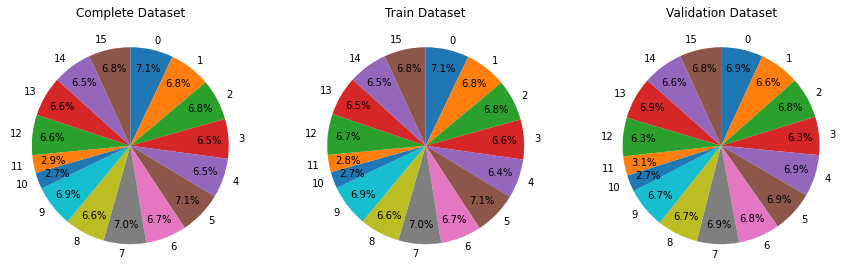
\includegraphics[width=0.4\textwidth]{images/DataBalance}
  \caption{Die verschiedenen Datensätze}
  \Description{}
  \label{fig:TrainingsDaten}
\end{figure}
\subsubsection{\normalfont{Mel-Spektrogramm}}
Ein Mel-Spektrogramm ist eine Repräsentation des Kurzzeitenergiespektrums eines Tons in Abhängigkeit des menschlichen Gehörs (siehe Abb.~\ref{fig:MelSpektrogramm}). Damit diese Abhängigkeit simuliert werden kann, wird die Frequenz an die Mel-Skala\cite{ganchev2005comparative} angepasst (siehe Formel ~\ref{MelFormel}). Es simuliert durch Filterbänke wie das menschliche Gehör einen Ton wahrnimmt und hebt somit die wichtigen Frequenzen an und schwächt jene Frequenzen ab, die nicht wahrgenommen werden. 
\begin{figure}[ht]
  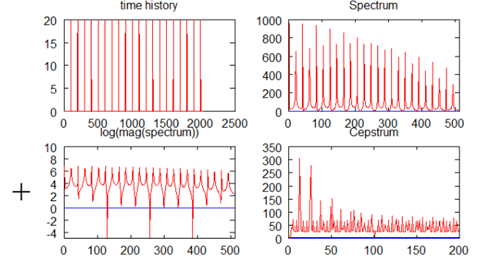
\includegraphics[width=0.45\textwidth]{images/melexplanation}
  \caption{Unterschiedliche Darstellungsmöglichkeiten von Audio}
  \Description{}
  \label{fig:MelSpektrogramm}
\end{figure}

\newpage
\begin{equation}\label{MelFormel}
M(f)=1125ln(1+\frac{f}{700})
\end{equation}

\noindent Beim Cepstrum wird auf der x-Achse die „quefrency“ dargestellt. Die Quefrenz hat als Einheit die Zeit und kann als Maß für die Verschiebung von Mustern im Zeitbereich interpretiert werden.\\
\noindent Das fertige Mel-Spektrogramm kann schließlich auch als eine Art Textur dargestellt werden, siehe Abb.\ref{fig:MelTextur}.  
Hier beschreibt die Farbe die Intensität, die X-Achse die Quefrenz und die Y-Achse die Frequenzbänder. 
\begin{figure}[ht]
  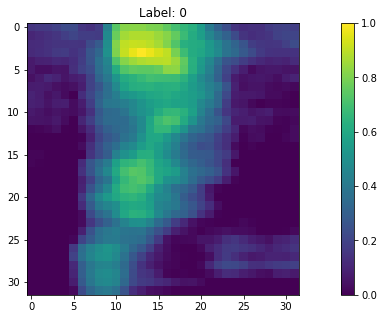
\includegraphics[width=0.45\textwidth]{images/Mel}
  \caption{Mel-Spektrogramm als Textur}
  \Description{}
  \label{fig:MelTextur}
\end{figure}


\subsection{Anwendungsumgebung}
Die Anwendungsumgebung in Unity stellt die Daten in dem gleichen Format wie die Trainingsumgebung bereit. Statt die Ausgabe, wie beim Trainingsprozess,  mit Labeln zu vergleichen, werden die Ergebnisse hier interpretiert, sodass in Unity ein Befehl ausgeführt werden kann. Die Daten werden in Unity mit einem Mircrophone Input erzeugt. Die Aufnahmen werden nach Worten getrennt, wodurch es möglich ist, die Worte einzeln zu klassifizieren. Dies ist vergleichbar damit, dass Worte im Datensatz als einzelne Dateien hinterlegt sind. 

\subsubsection{\normalfont{Deployment}}
Mit dem Barracuda Package ist es möglich, neuronale Netze in Unity zu verwenden. Das Plugin kann Netze im eigenen Format .nn, sowie im Austauschformat .onnx einlesen und anwenden. Dabei werden noch nicht alle Funktionalitäten des ONNX-Formats komplett unterstützt. Für die Anwendung einfacher feedforward Netze ist die Komptabilität allerdings weitestgehend gegeben. Den Trainingsprozess konnten wir so mit dem Machine Learning Framework PyTorch durchführen und die Netze mit den entsprechenden Trainingständen als ONNX exportieren. Abb. \ref{fig:UnityApp} zeigt die Demo-Anwendung in Unity, welche die Anwendungsumgebung aus Kapitel \ref{section:Umgebung} darstellt. 

\subsubsection{\normalfont{Audio Slicing}}
In dem Notebook “FeatureDetection” \footnote[1]{https://github.com/Alpe6825/Unicornn/blob/master/slicingShowcase/Feature\\Detection.ipynb}  ist der Vorgang zur Verdeutlichung  in Python umgesetzt worden. In der Anwendung läuft dies über ein C\#-Script. 
\newline
\newline
\noindent Der Algorithmus: 
\begin{itemize}
\item Einlesen der .wav
\item Konvertieren in eine Liste aus Buffern (Custom Class)
\item Iterieren durch die Buffer-Liste und eine Serie aus "lauten" \ Buffern finden
\item Die Serie an "lauten" \ Buffern in vorherige und folgende Buffer einbetten
\item Die Buffer-Liste wieder in eine Float-Liste konvertieren
\end{itemize}

\noindent Es gibt Einstellungsmöglichkeiten, mit denen man die Genauigkeit anpassen könnte. Zum Beispiel die Größe der Buffer verringern oder den Threshold verändern.
Dies funktioniert relativ zuverlässig und hat nur bei den Wörter "forward$"$ und "backward" \ Probleme, wahrscheinlich weil dort beim Sprechen eine kleine Pause im Wort vorhanden ist. Dem kann man entgegenwirken indem man die Buffersize erhöht. \\
Abb.\ref{fig:Audio} zeigt die gesamte Audiospur, Abb.\ref{fig:Audio1} und Abb.\ref{fig:Audio2} zeigen die einzelnen getrennten Worte.

\begin{figure}[ht]
  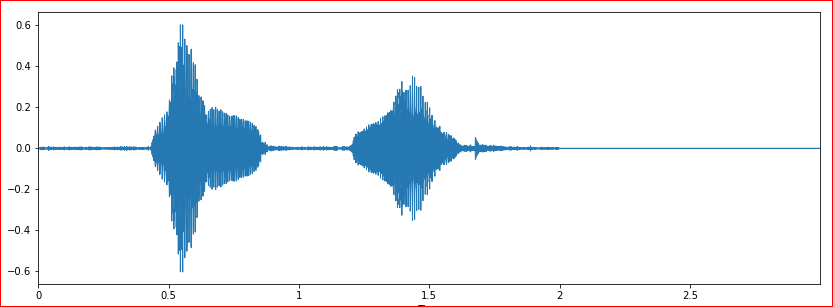
\includegraphics[width=0.3\textwidth]{images/Audio1}
  \caption{Waveform der gesamten Audiospur.}
  \Description{}
  \label{fig:Audio}
\end{figure} 
\begin{figure}[ht]
  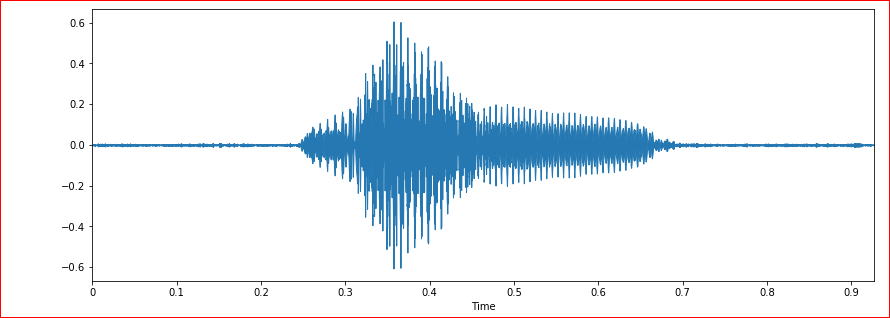
\includegraphics[width=0.3\textwidth]{images/Audio2}
  \caption{Waveform des ersten Wortes.}
  \Description{}
  \label{fig:Audio1}
\end{figure} 
\begin{figure}[ht]
  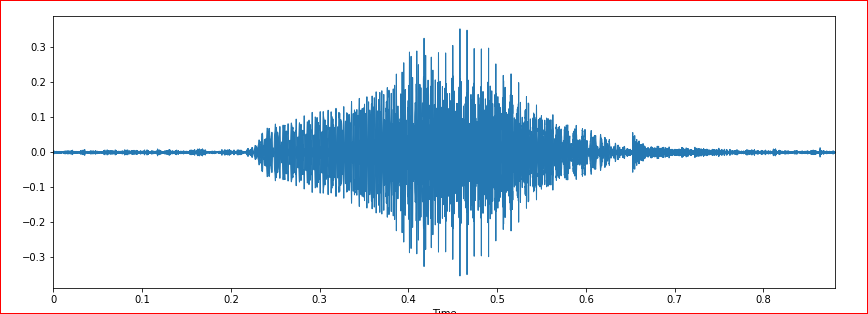
\includegraphics[width=0.3\textwidth]{images/Audio3}
  \caption{Waveform des zweiten Wortes.}
  \Description{}
  \label{fig:Audio2}
\end{figure} 

\section{Agent}
Da sich das Mel-Spektrogramm als Bild handhaben lässt, bietet sich die Verwendung von 2D-Convolutional Neural Networks an. Grundlegend lässt sich die Verarbeitung der Bilder durch CNNs in zwei Abschnitte einteilen: Feature Erkennung und Klassifizierung.\\
Die Feature Erkennung dient dazu durch zweidimensionale Faltungen markante Strukturen zu erkennen, welche für bestimmte Klassen typisch sind. Die Werte der Faltungsmatrizen werden im Training erlernt. Zur Reduzierung der Auflösung von Featuremaps wird der Maxpooling Algorithmus mit einer Kernelgröße von 2x2 (Halbierung der Auflösung) verwendet. Von vier Pixeln wird dabei lediglich der Pixel mit dem größten Wert übernommen. Als Aktivierungsfunktion wird typischerweise die ReLu-Funktion verwendet (siehe Formel~\ref{ReLu}). 


\begin{equation}\label{ReLu}
ReLu(x) = max(0,x)
\end{equation}


\noindent Die ReLu-Funktion besitzt keine Obergrenze. Um zu verhindern, dass Werte im Laufe des Netzes stark gestreut werden, kommen Batch-Normalisierungs-Layer \cite{ioffe2015batch} zwischen den Faltungen zum Einsatz. 
Die Klassifizierung besteht typischerweise aus vollverbundenen Schichten. Aufgabe ist es auf Basis von vielen gering aufgelösten Featuremaps (Ausgabe des ersten Abschnittes) für jede Klasse einen Score zu errechnen. Letztendlich wird sich bei der Klassenvorhersage dann für die Klasse mit dem höchsten Score entschieden. 
Für die Klassifikation wurden ein VGG19 und ein ResNet verwendet. Beim VGG handelt es sich um ein neuronales Netzwerk, bei dem die Output-Werte eines Layers als Input-Werte in das darauffolgende Layer gegeben werden. Im Unterschied dazu können bei einem ResNet vor der Eingabe dieser Werte in ein Layer noch Input-Werte vorheriger Layer aufsummiert werden, wodurch ein tieferes Netzwerk entsteht. 

\section{Training}
\label{section:training}
Beide Netze wurden über 20 Epochen trainiert. Als Loss Funktion wurde der, für Klassifizierungsprobleme oft verwendende, CrossEntropy-Loss verwendet. Der Loss-Wert wurde, bei einer Batchgröße von 128, pro Batch gemittelt.  
Um den Trainingsprozess qualitativ bewerten zu können wird nach jeder Epoche der Testdatensatz durch das Netz gespeist. Auf Basis dessen wird, neben der Berechnung eines Loss-Wertes zur Anpassung der Learningrate, überprüft, in wie vielen Fällen die Klassifizierung korrekt liegt.  Ein Accuracy-Wert von 1 repräsentiert dabei den Fall, dass die Klassifizierung für alle Testdaten erfolgreich war. Ein Wert von 0 das keine Klassifizierung korrekt war. 
Der Trainingsprozess wurde pro Netz mit dem SGD- sowie dem Adam-Optimizer durchlaufen. Letzterer führte bei beiden Netzen zu besseren Ergebnissen. Die Accuracy stieg bei beiden Netzen mit dem Adam Optimizer innerhalb von nur weniger Epochen auf über 90\%, siehe Abb. \ref{fig:VGG_Adam} und Abb. \ref{fig:ResNet_Adam}. Mit dem SGD-Optimizer konnte in keinem der beiden Netze eine Accuracy von über 90\% innerhalb von 20 Epochen erreicht werden, siehe Abb. \ref{fig:VGG_SGD} und Abb. \ref{fig:ResNet_SGD}.
\newline
\newline
Die Learningrate war zu Beginn der Trainingsdurchläufe je 0,001. Für den Fall, dass sich der Loss-Wert für die Testdaten über 5 Epochen nicht markant ändert (<0.0001) wurde die Learningrate um den Faktor 10 verkleinert. 

\section{Auswertung}
Basierend auf den Loss und Accuracy-Verläufen der Testdaten im Anhang \ref{section:Anhang} schien die Verwendung des Adam-Optimizers zu besseren Ergebnissen beider Netze, sowohl bei den Loss- als auch bei den Accuracy-Werten zu führen. Insgesamt schien das VGG19 Netz mit Batch Normalisierung die besten Ergebnisse liefern zu können.  
\newline
\newline
Die folgende Confusion-Matrix in Abb.\ref{fig:Confusion-Matrix_VGG_Adam} zeigt die entsprechenden Ergebnisse der Testdaten. In den meisten Fällen verteilen sich alle Fehlklassifizierungen gleichmäßig auf alle anderen Klassen. Ausnahme bildet das Wort ,,four“ dies neigt bei einer Fehleinschätzung tendenziell etwas näher zur Klassifizierung als ,,forward“. Grund dafür ist mit hoher Wahrscheinlichkeit die phonetische Ähnlichkeit der beiden Worte.

\begin{figure}[ht]
  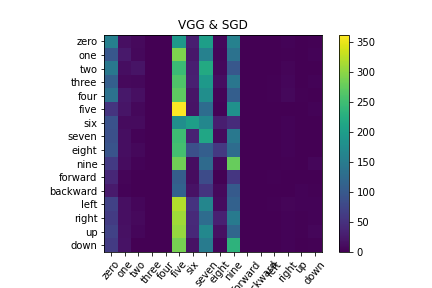
\includegraphics[width=0.5\textwidth]{images/Confusion-Matrix_VGG_SGD}
  \caption{VGG und SGD}
  \Description{}
  \label{fig:Confusion-Matrix_VGG_SGD}
\end{figure} 

\begin{figure}[ht]
  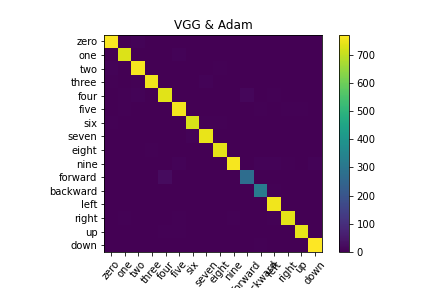
\includegraphics[width=0.5\textwidth]{images/Confusion-Matrix_VGG_Adam}
  \caption{VGG und Adam}
  \Description{}
  \label{fig:Confusion-Matrix_VGG_Adam}
\end{figure} 

\newpage
\begin{figure}[ht]
  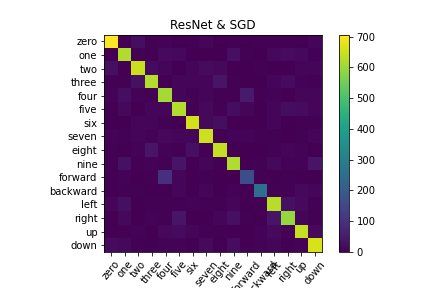
\includegraphics[width=0.5\textwidth]{images/Confusion-Matrix_ResNet_SGD}
  \caption{ResNet und SGD}
  \Description{}
  \label{fig:Confusion-Matrix_ResNet_SGD}
\end{figure} 

\begin{figure}[ht]
  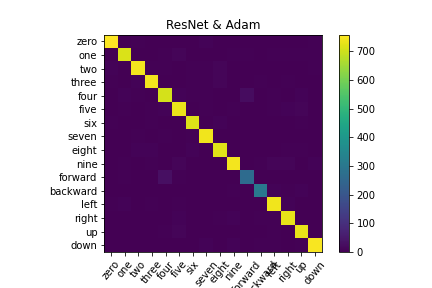
\includegraphics[width=0.5\textwidth]{images/Confusion-Matrix_ResNet_Adam}
  \caption{ResNet und Adam}
  \Description{}
  \label{fig:Confusion-Matrix_ResNet_Adam}
\end{figure} 

\noindent Des Weiteren scheint es als würden die Worte ,,forward“ und ,,backward“ weniger gut erkannt werden als die restlichen Wörter. In Tabelle \ref{table:data} wird deutlich, dass für zwei der Klassen weniger Beispiele vorliegen. Bei diesen handelt es sich um die Worte ,,forward“ und ,,backward“.
\newline
\newline

\begin{table}[ht]
\centering
\begin{tabular}{|l|c|l|c|}
\hline
zero & 4052 & eight & 3787  \\
\hline
one & 3890 & nine & 3934  \\
\hline
two & 3880 & forward & 1557  \\
\hline
three &  3727 & backward & 1664 \\
\hline
four & 3728 & left & 3801 \\
\hline
five & 4052 & Right & 3779\\
\hline
six & 3860 & up & 3723\\
\hline
seven & 3998 & down & 3917\\
\hline
\end{tabular}
\caption{Anzahl der Daten im Datensatz von Warden\cite{speechcommandsv2}.}
\label{table:data}
\end{table}

\noindent Ursprünglich war eine größere Varianz an Wortkombinationsmöglichkeiten geplant. Dazu wurden bereits Sprachaufnahmen von den Worten der folgenden Wörten gesammelt: 
\newline
\newline
„create“, „delete“, „select“, „color“, „move“, „cube“, „sphere“, „plane“, „red“, „green“, „blue“, „white“. 
\newline
\newline
Pro Wort kamen insgesamt 147 Aufnahmen zusammen. Daraufhin war geplant diese mit Hilfe von Audio-Modulationen (u.a. Hall, Pitch, Verschiebung) zu verändern und so auf ca. 1500 Aufnahmen zu erweitern. Durch die Verwendung von zufälligen Werten bei den Modulationen sollten Korrelationen, die durch gleiche Modulations-Funktionen entstehen und zu Fehlklassifikationen führen könnten, verhindert werden.\\
Bislang gelang es nicht eine Verzehnfachung ohne Korrelation zu erzeugen.

\section{Fazit \& Ausblick}
Wir haben einen Sprachassistent für Unity 3D entwickelt, der in seiner Funktionsweise derzeit noch stark begrenzt ist, dafür aber solide funktioniert. Eine Skalierung ist bei entsprechender Anzahl von Trainingsdaten durchaus denkbar. Eine mögliche Erweiterung könnte zukünftig darin bestehen, RNNs oder LSTMs für die Verarbeitung von kontinuierlichen Inputsequenzen zu verwenden.
\newline
\newline
Derzeit wird die Berechnung des Spektrogramms noch in Python durchgeführt, da in Unity 3D keine entsprechenden Funktionen bereitstehen. Der Umweg über ein Python-Script im Hintergrund kann derzeit noch als Bottleneck der Pipeline betrachtet werden und wäre für eine Auslieferung des Programms bislang nicht optimal. Eine vollständige Verarbeitung der Daten in Unity steht noch aus. 
\newline
\newline
Die Beschaffung und notwendige Menge an Trainingsdaten hat sich als problematischster Punkt des Projektes herausgestellt.

\bibliographystyle{ACM-Reference-Format}
\bibliography{literatur.bib}

\newpage
\onecolumn
\appendix
\section{Anhang}
\label{section:Anhang}
\begin{figure}[H]
  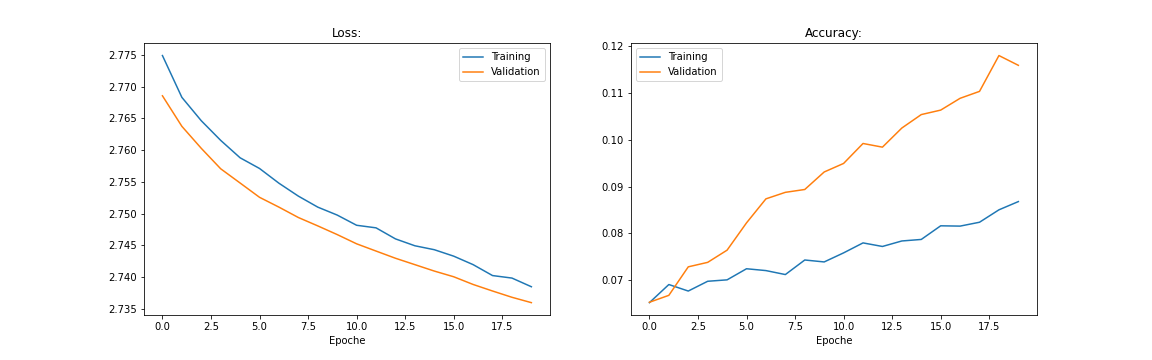
\includegraphics[width=0.7\textwidth]{images/Loss_Acc_VGG_SGD}
  \caption{Loss Accuracy von VGG \& SGD}
  \Description{}
  \label{fig:VGG_SGD}
\end{figure} 

\begin{figure}[H]
  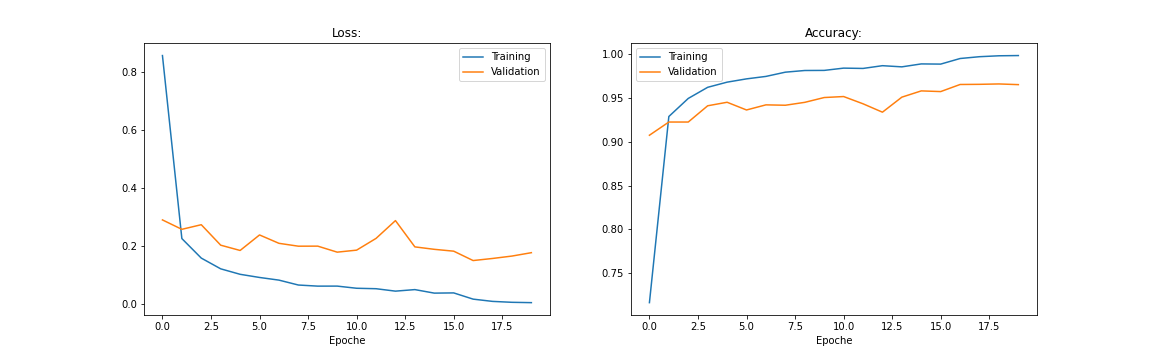
\includegraphics[width=0.7\textwidth]{images/Loss_Acc_VGG_Adam}
  \caption{Loss Accuracy von VGG \& Adam}
  \Description{}
  \label{fig:VGG_Adam}
\end{figure} 

\begin{figure}[H]
  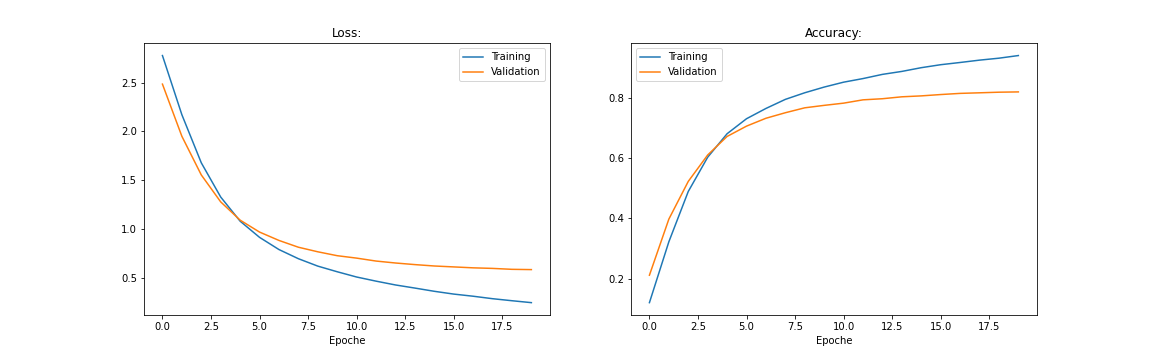
\includegraphics[width=0.7\textwidth]{images/Loss_Acc_ResNet_SGD}
  \caption{Loss Accuracy von ResNet \& SGD}
  \Description{}
  \label{fig:ResNet_SGD}
\end{figure} 

\begin{figure}[H]
  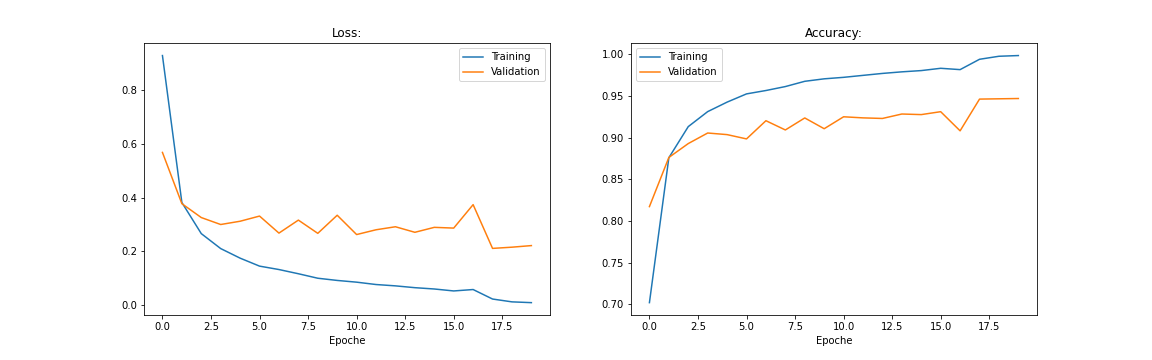
\includegraphics[width=0.7\textwidth]{images/Loss_Acc_ResNet_Adam}
  \caption{Loss Accuracy von ResNet \& Adam}
  \Description{}
  \label{fig:ResNet_Adam}
\end{figure} 

\end{document}
\endinput
